% Présentation A2 de tout le projet : cadre, baseline, Données, Entraînement, Inférence, combinaisons, bilan.
% Ce qui n'a pas encore de résultats est un trou visible, \trou{largeur}{hauteur}{ce qu'il faudra y mettre} : à
% remplacer par la figure, puis retirer \afaire du titre.
% Règles suivies : un message par slide, formulé dans le titre ; la figure est la preuve ; le protocole de chaque
% chiffre est indiqué en bas de la slide (consignes du cours, slides 84, 86 et 89 : 16:9, 5 minutes).
%
% Compiler depuis ce dossier :   pdflatex presentation.tex  (deux fois)
% Figures de la baseline :       python slides/make_figures.py --weights <dossier> (depuis la racine du repo)
\documentclass[aspectratio=169,11pt]{beamer}
\usepackage[utf8]{inputenc}
\usepackage[T1]{fontenc}
\usepackage{lmodern}
\usepackage[french]{babel}
\usepackage{amsmath,booktabs,tikz}
\usetikzlibrary{arrows.meta,positioning,calc,babel}
\graphicspath{{figures/}}

\definecolor{ink}{HTML}{0B0B0B}
\definecolor{muted}{HTML}{52514E}
\definecolor{accent}{HTML}{2A78D6}
\definecolor{warm}{HTML}{EB6834}
\definecolor{panel}{HTML}{EEF4FC}
\definecolor{surface}{HTML}{FCFCFB}

\setbeamercolor{background canvas}{bg=surface}
\setbeamercolor{normal text}{fg=ink}
\setbeamercolor{frametitle}{fg=ink}
\setbeamercolor{title}{fg=ink}
\setbeamercolor{subtitle}{fg=muted}
\setbeamercolor{author}{fg=muted}
\setbeamercolor{itemize item}{fg=accent}
\setbeamerfont{frametitle}{size=\large,series=\bfseries}
\setbeamerfont{title}{size=\LARGE,series=\bfseries}
\setbeamertemplate{navigation symbols}{}
\setbeamertemplate{itemize item}{\small$\bullet$}
\setbeamertemplate{footline}{%
  \hspace{1em}{\scriptsize\color{muted}\insertsection}\hfill
  {\scriptsize\color{muted}\insertframenumber}\hspace{1em}\vspace{0.5em}}

% Protocole de la mesure, ou référence, en bas de slide.
\newcommand{\source}[1]{\vfill{\scriptsize\color{muted}#1\par}}
% Emplacement réservé à un résultat pas encore obtenu.
\newcommand{\trou}[3]{\tikz\node[draw=warm, dashed, line width=0.9pt, rounded corners=3pt, minimum width=#1, minimum height=#2,
  text width=#1-5mm, align=center, font=\small, text=warm]{\textbf{À compléter}\\#3};}
% Marque, dans le titre, une slide dont les résultats manquent.
\newcommand{\afaire}{{\color{warm}\normalsize\ [à compléter]}}

\title{À générateur imposé, que peut-on gagner ?}
\subtitle{GAN sur MNIST : données, entraînement et inférence}
\author{Quentin Revillon, Noé Mosca, Nicodème Gorge\\Groupe 3}
\date{}

\begin{document}

\begin{frame}[plain,noframenumbering]
  \titlepage
\end{frame}

% ------------------------------------------------------------------------------------------------------------
\section{Cadre}

\begin{frame}{Le générateur est imposé : trois leviers restent}
  \centering\vspace{0.6em}
  \begin{tikzpicture}[
      box/.style={draw=muted, rounded corners=3pt, minimum height=11mm, align=center, font=\small, fill=white},
      lever/.style={rounded corners=3pt, minimum height=12mm, minimum width=33mm, align=center, font=\small, fill=panel},
      arr/.style={-{Stealth[length=2.2mm]}, muted, line width=0.7pt}]
    \node[box, minimum width=20mm] (z) {$z \in \mathbb{R}^{100}$};
    \node[box, minimum width=46mm, right=9mm of z, line width=1pt] (g) {$G$ : MLP imposé\\$100 \to 256 \to 512 \to 1024 \to 784$};
    \node[box, minimum width=20mm, right=9mm of g] (x) {image\\$28 \times 28$};
    \draw[arr] (z) -- (g);
    \draw[arr] (g) -- (x);
    \node[lever, below=11mm of z, xshift=4mm] (data) {\textbf{Données}\\Nicodème};
    \node[lever, below=11mm of g] (train) {\textbf{Entraînement}\\Noé};
    \node[lever, below=11mm of x, xshift=-4mm] (inf) {\textbf{Inférence}\\Quentin};
    \path (g.south west) -- (g.south east) coordinate[pos=0.2] (gleft) coordinate[pos=0.8] (gright);
    \draw[arr, accent] (data) -- (gleft);
    \draw[arr, accent] (train) -- (g);
    \draw[arr, accent] (inf) -- (gright);
  \end{tikzpicture}

  \vspace{1.3em}
  {\large À architecture fixée, qu'améliore chaque levier : la \textbf{qualité} ou la \textbf{diversité} ?}
\end{frame}

\begin{frame}{Méthode proposée : séparer entraînement, choix et chiffres finaux}
  \centering\vspace{0.4em}
  \begin{tikzpicture}[
      box/.style={draw=muted, rounded corners=3pt, minimum height=11mm, minimum width=27mm, align=center, font=\small, fill=white},
      use/.style={rounded corners=3pt, minimum height=11mm, minimum width=42mm, align=center, font=\small, fill=panel},
      arr/.style={-{Stealth[length=2.2mm]}, muted, line width=0.7pt}]
    \node[box] (val) {\textbf{val}\\10 000};
    \node[box, above=3mm of val] (train) {\textbf{train}\\50 000};
    \node[box, below=3mm of val] (test) {\textbf{test}\\10 000};
    \path (train) -- (val) coordinate[midway] (split);
    \node[box, left=24.5mm of split] (mnist) {MNIST train\\60 000};
    \node[box, left=11mm of test] (mnistt) {MNIST test\\10 000};
    \node[use, right=11mm of train] (u1) {entraîner $G$ et $D$};
    \node[use, right=11mm of val] (u2) {choisir époque et réglages};
    \node[use, right=11mm of test] (u3) {chiffres finaux, une seule fois};
    \draw[arr] (mnist) -- (train);
    \draw[arr] (mnist) -- (val);
    \draw[arr] (mnistt) -- (test);
    \draw[arr] (train) -- (u1);
    \draw[arr] (val) -- (u2);
    \draw[arr] (test) -- (u3);
  \end{tikzpicture}

  \vspace{1em}
  {\small \textbf{Une seule variable à la fois.} \textbf{Mesures :} FID, précision, rappel, grilles d'images.\\[0.3em]
   \textbf{Reproductible :} pertes identiques sur 50 époques, entre deux nœuds GPU différents.}
  \source{``Never tune on the test set'' (cours Slurm). Protocole : slide 84 du cours. Appliqué à la baseline uniquement : les volets Données et Entraînement utilisent encore les 60\,000 images, sans validation.}
\end{frame}

% ------------------------------------------------------------------------------------------------------------
\section{Baseline}

\begin{frame}{Baseline : le FID n'atteint son minimum que vers l'époque 120}
  \centering
  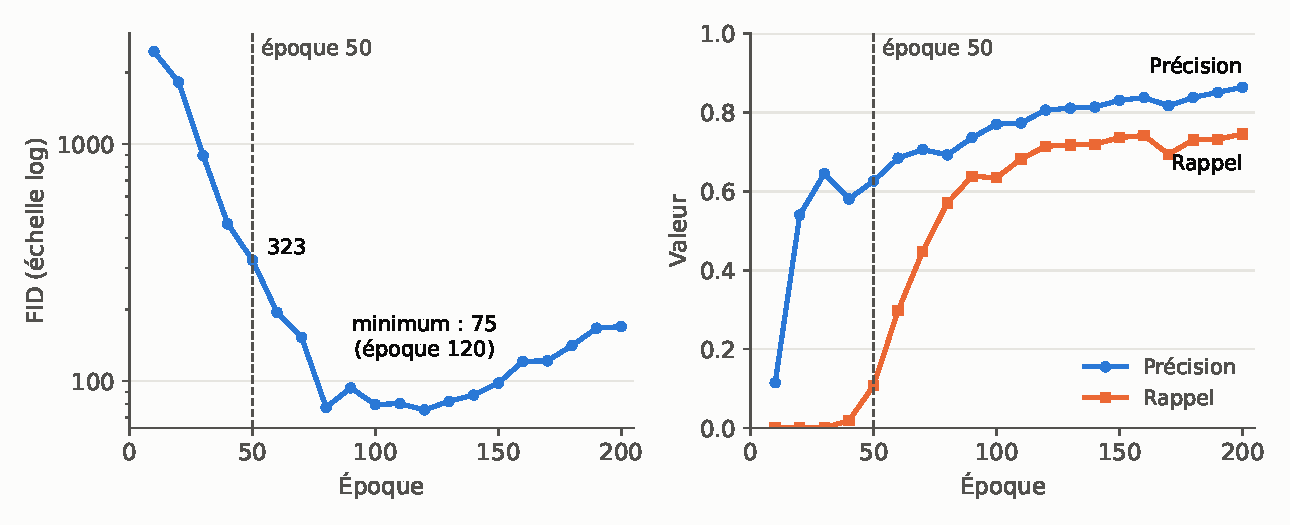
\includegraphics[width=\linewidth]{baseline_curves.pdf}
  \source{Réglages du code fourni (BCE, lr $2\cdot10^{-4}$), batch 100, 50\,000 images. Petit CNN MNIST, contre val ; évaluation toutes les 10 époques ; une seule graine.}
\end{frame}

\begin{frame}{Baseline : après l'époque 120, les classes se déséquilibrent}
  \centering\vspace{-0.6em}
  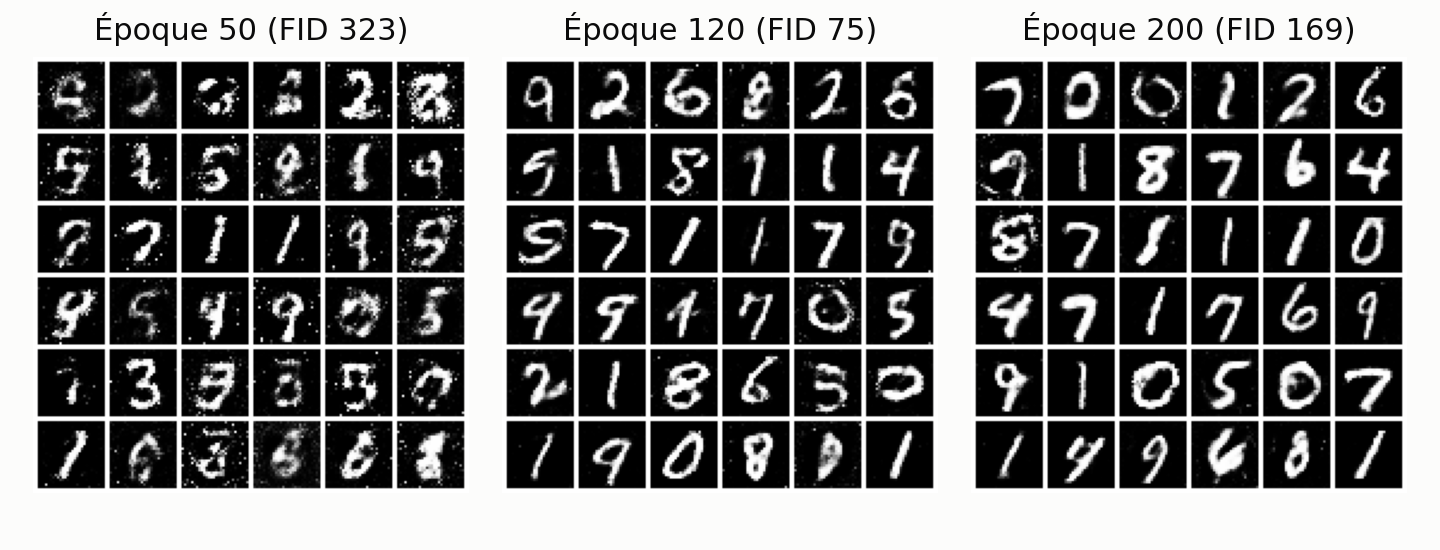
\includegraphics[width=0.68\linewidth]{baseline_grids.png}\\[-0.3em]
  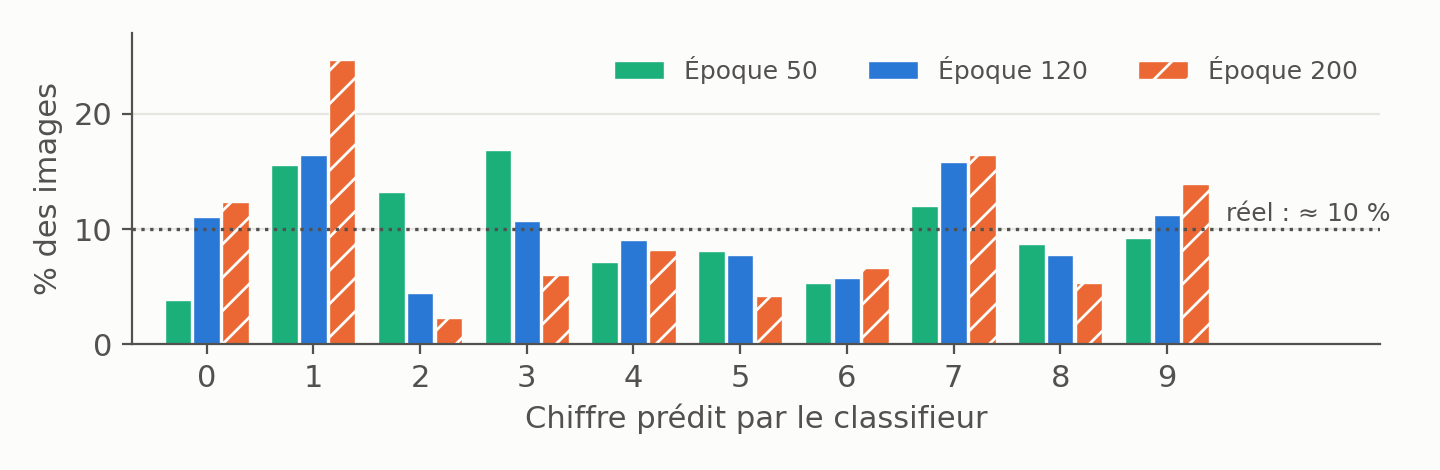
\includegraphics[width=0.68\linewidth]{baseline_classes.png}
  \source{Mêmes $z$ dans les trois grilles. Époque 200 : 24,7\,\% de « 1 », 2,3\,\% de « 2 ». Petit CNN MNIST, contre val.}
\end{frame}

% ------------------------------------------------------------------------------------------------------------
\section{Données}

\begin{frame}{Données : entraîner sur les images denses, bruiter les entrées de $D$\afaire}
  \vspace{0.3em}
  \begin{columns}[T,onlytextwidth]
    \column{0.47\textwidth}\centering
    \textbf{Sélection d'instances}\\[0.2em]
    {\small ne garder que les images les plus denses}\\[0.6em]
    \trou{62mm}{33mm}{Grilles et FID, précision, rappel\\selon la fraction gardée (50\,\%, 75\,\%)}
    \column{0.47\textwidth}\centering
    \textbf{Bruit d'instance}\\[0.2em]
    {\small ajouter un bruit gaussien aux entrées de $D$}\\[0.6em]
    \trou{62mm}{33mm}{Grilles et FID, précision, rappel\\selon le niveau de bruit (0,1 ; 0,3)}
  \end{columns}
  \source{DeVries et al. 2020 ; Sønderby et al. 2017. Volet de Nicodème : 9 configurations, 3 graines, 60\,000 images sans validation. Résultats à reporter ici.}
\end{frame}

% ------------------------------------------------------------------------------------------------------------
\section{Entraînement}

\begin{frame}{Entraînement : à 50 époques, une perte relativiste divise le FID par 4}
  \centering\vspace{-0.3em}
  {\small $\displaystyle \mathcal{L}_D = \mathrm{softplus}\big(D(G(z)) - D(x)\big) + \frac{\gamma}{2}\big(\underbrace{\|\nabla_x D(x)\|^2}_{R_1} + \underbrace{\|\nabla_x D(G(z))\|^2}_{R_2}\big)$}\\[0.3em]
  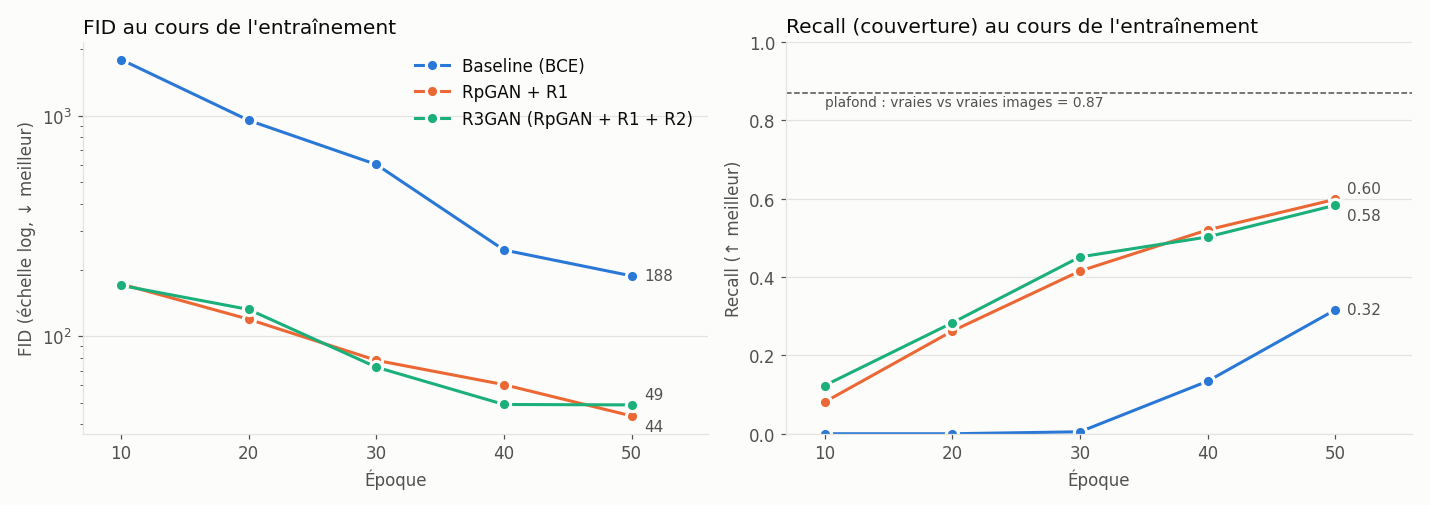
\includegraphics[width=0.82\linewidth]{noe_fid_recall_curves.png}
  \source{Huang et al., \emph{The GAN is dead; long live the GAN!}, NeurIPS 2024 : seule la perte est reprise. Runs de Noé : 60\,000 images, petit CNN MNIST, contre MNIST test, une seule graine. Sa baseline à 50 époques n'a pas convergé.}
\end{frame}

\begin{frame}{Entraînement : sans R1 la perte diverge, avec les bêtas du papier elle s'effondre}
  \centering\vspace{0.5em}
  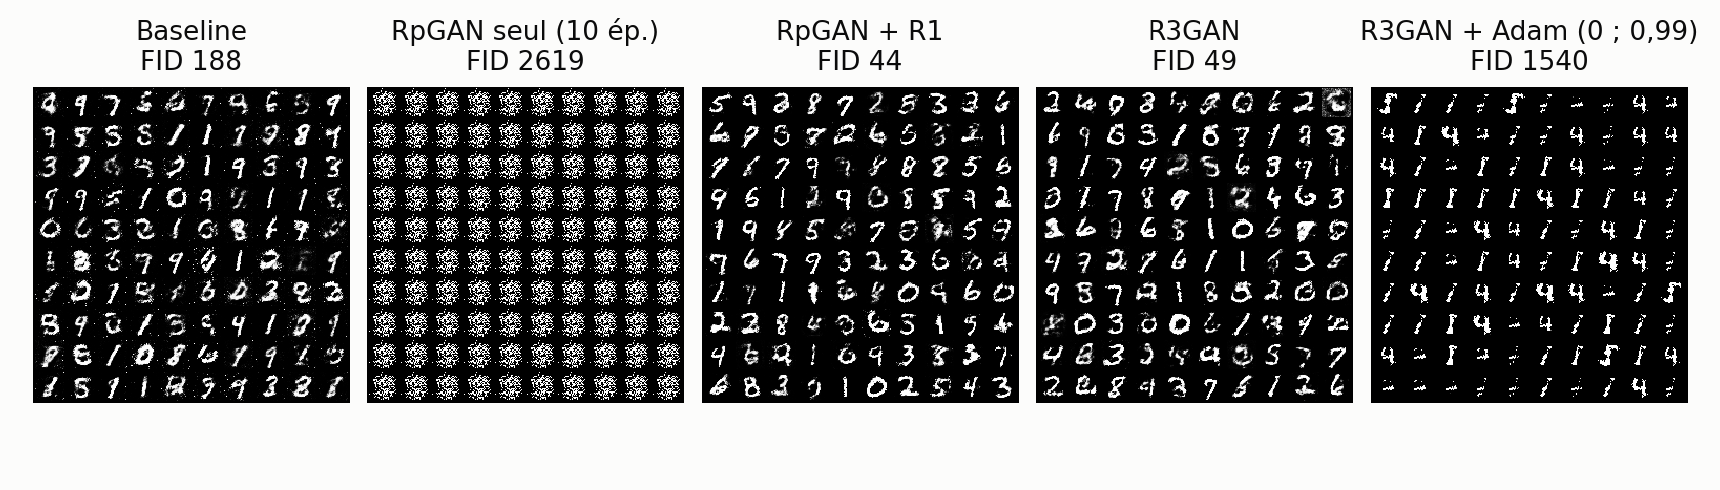
\includegraphics[width=\linewidth]{noe_ablation.png}

  \vspace{0.6em}
  {\small \textbf{Une seule modification à chaque colonne.} Coût mesuré : +5 à 10\,\% de temps par époque.}
  \source{Runs de Noé : 50 époques (10 pour RpGAN seul), petit CNN MNIST, contre MNIST test, une seule graine.}
\end{frame}

% ------------------------------------------------------------------------------------------------------------
\section{Inférence}

\begin{frame}{Inférence : rejeter les images que $D$ juge irréalistes\afaire}
  \centering\vspace{-0.2em}
  {\small $\displaystyle \frac{p_d(x)}{p_g(x)} = e^{\tilde D(x)}
    \qquad p_{\mathrm{accept}}(x) = \sigma\big(\tilde D(x) - \tilde D_M - \log(1 - e^{\tilde D(x) - \tilde D_M - \epsilon}) - \gamma\big)$}\\[0.7em]
  \begin{columns}[T,onlytextwidth]
    \column{0.47\textwidth}\centering
    \trou{62mm}{33mm}{FID, précision, rappel selon le percentile de $\gamma$ : $D$ brut contre $D$ réentraîné}
    \column{0.47\textwidth}\centering
    \trou{62mm}{33mm}{Images gardées et rejetées, taux d'acceptation, temps de génération}
  \end{columns}
  \source{Azadi et al. 2019 (DRS), implémenté avec KeepTraining. Mesure en attente de GPU sur Juliet. À rapporter : acceptation, temps, lot complet (slide 82 du cours).}
\end{frame}

% ------------------------------------------------------------------------------------------------------------
\section{Combinaisons}

\begin{frame}{Combinaisons : chaque levier seul, puis ensemble\afaire}
  \centering\vspace{0.8em}
  \begin{tabular}{lcccc}
    \toprule
    & FID & Précision & Rappel & Coût \\
    \midrule
    Baseline, époque 120 & \color{warm}? & \color{warm}? & \color{warm}? & \color{warm}? \\
    + Données & \color{warm}? & \color{warm}? & \color{warm}? & \color{warm}? \\
    + Entraînement & \color{warm}? & \color{warm}? & \color{warm}? & \color{warm}? \\
    + Inférence & \color{warm}? & \color{warm}? & \color{warm}? & \color{warm}? \\
    Meilleure combinaison & \color{warm}? & \color{warm}? & \color{warm}? & \color{warm}? \\
    \bottomrule
  \end{tabular}

  \vspace{1em}
  {\small \textbf{Même split, même nombre d'époques, même mesure, plusieurs graines.}}
  \source{Consigne, slide 76 du cours : ``Compare each intervention separately, then useful combinations''. À mesurer sur test avec Inception et VGG.}
\end{frame}

% ------------------------------------------------------------------------------------------------------------
\section{Bilan}

\begin{frame}{Bilan : la durée et la perte comptent, le reste est à mesurer\afaire}
  \vspace{0.5em}
  \begin{columns}[T,onlytextwidth]
    \column{0.31\textwidth}
    \textbf{\color{accent}Établi}\\[0.5em]\small
    Durée : FID 323 $\to$ 75\\[0.4em]
    Perte : FID 188 $\to$ 44, rappel 0,32 $\to$ 0,60
    \column{0.31\textwidth}
    \textbf{\color{warm}À compléter}\\[0.5em]\small
    Effet des données\\[0.4em]
    Effet du rejet et son coût\\[0.4em]
    Meilleure combinaison
    \column{0.31\textwidth}
    \textbf{Limites actuelles}\\[0.5em]\small
    Une seule graine\\[0.4em]
    Protocoles différents : ne pas comparer 75 et 44\\[0.4em]
    Petit CNN, pas la mesure du classement
  \end{columns}
\end{frame}

% ------------------------------------------------------------------------------------------------------------
\appendix
\section{Annexe}

\begin{frame}{Annexe : le FID dépend du réseau, notre calcul Inception colle au classement}
  \centering
  $\displaystyle \mathrm{FID} = \|\mu_r - \mu_g\|^2 + \mathrm{Tr}\big(\Sigma_r + \Sigma_g - 2(\Sigma_r\Sigma_g)^{1/2}\big)$

  \vspace{1em}
  {\footnotesize
  \begin{tabular}{lccc}
    \toprule
    \texttt{checkpoints/G.pth} & Classement du prof & Inception + VGG (nous) & Petit CNN \\
    \midrule
    FID & 44,0 & \textbf{43,0} $\pm$ 0,4 & 103,7 \\
    Précision & 0,705 & 0,400 $\pm$ 0,004 & 0,804 \\
    Rappel & 0,502 & 0,454 $\pm$ 0,006 & 0,749 \\
    \bottomrule
  \end{tabular}}

  \vspace{1em}
  {\small Le FID est calé. La précision et le rappel ne le sont pas encore.}
  \source{Référence : MNIST test pour nos deux colonnes ; non précisée pour le classement. Inception + VGG : 3 graines, k = 5, 9\,984 images pour P/R. Petit CNN : k = 3, une évaluation. FID : Heusel et al. 2017. P/R : Kynkäänniemi et al. 2019. Classifieur MNIST pour P/R : Issenhuth et al. 2021.}
\end{frame}

\end{document}
